\section{ПІДХІД ГЛИБОКОГО НАВЧАННЯ У ПОБУДОВІ РЕКОМЕНДАЦІЙ}
Моделі і алгоритми глибокого навчання на основі штучних нейронних мереж в останні роки знаходять своє використання у багатьох прикладних сферах інформатики. Цей підхід також показав прекрасні результати у порівнянні із класичними моделями у задачах побудови рекомендацій,що є наслідком уміння нейромереж знаходитити не лінійні і не тривіальні зв’язки у навчальних даних. А також, можливість використання в якості джерела даних як візуальну, так і текстову, контекстну інформацію. Розглянемо класичну структуру нейронної мережі.


\subsection{Нейронна мережа прямого поширення}
Перцептрон - математична модель яка відтворює сприйняття інформації за подобою мозку людини.Елементарний перцептрон складається з трьох типів елементів: S-елементів, А-елементів та одного R-елемента (Рис 3.1). S - це шар датчиків або рецепторів. У фізичному варіанті вони відповідають, наприклад, до схожих чутливих клітин сітківки ока або фоторезисторів матриці фотокамери. Кожен рецептор може бути в одному з двох станів - спокою або збудження, і лише в останньому випадку він передає сигнал до наступного шару і іншим  повязаним елементам.
\begin{figure}[H]
    \centering
    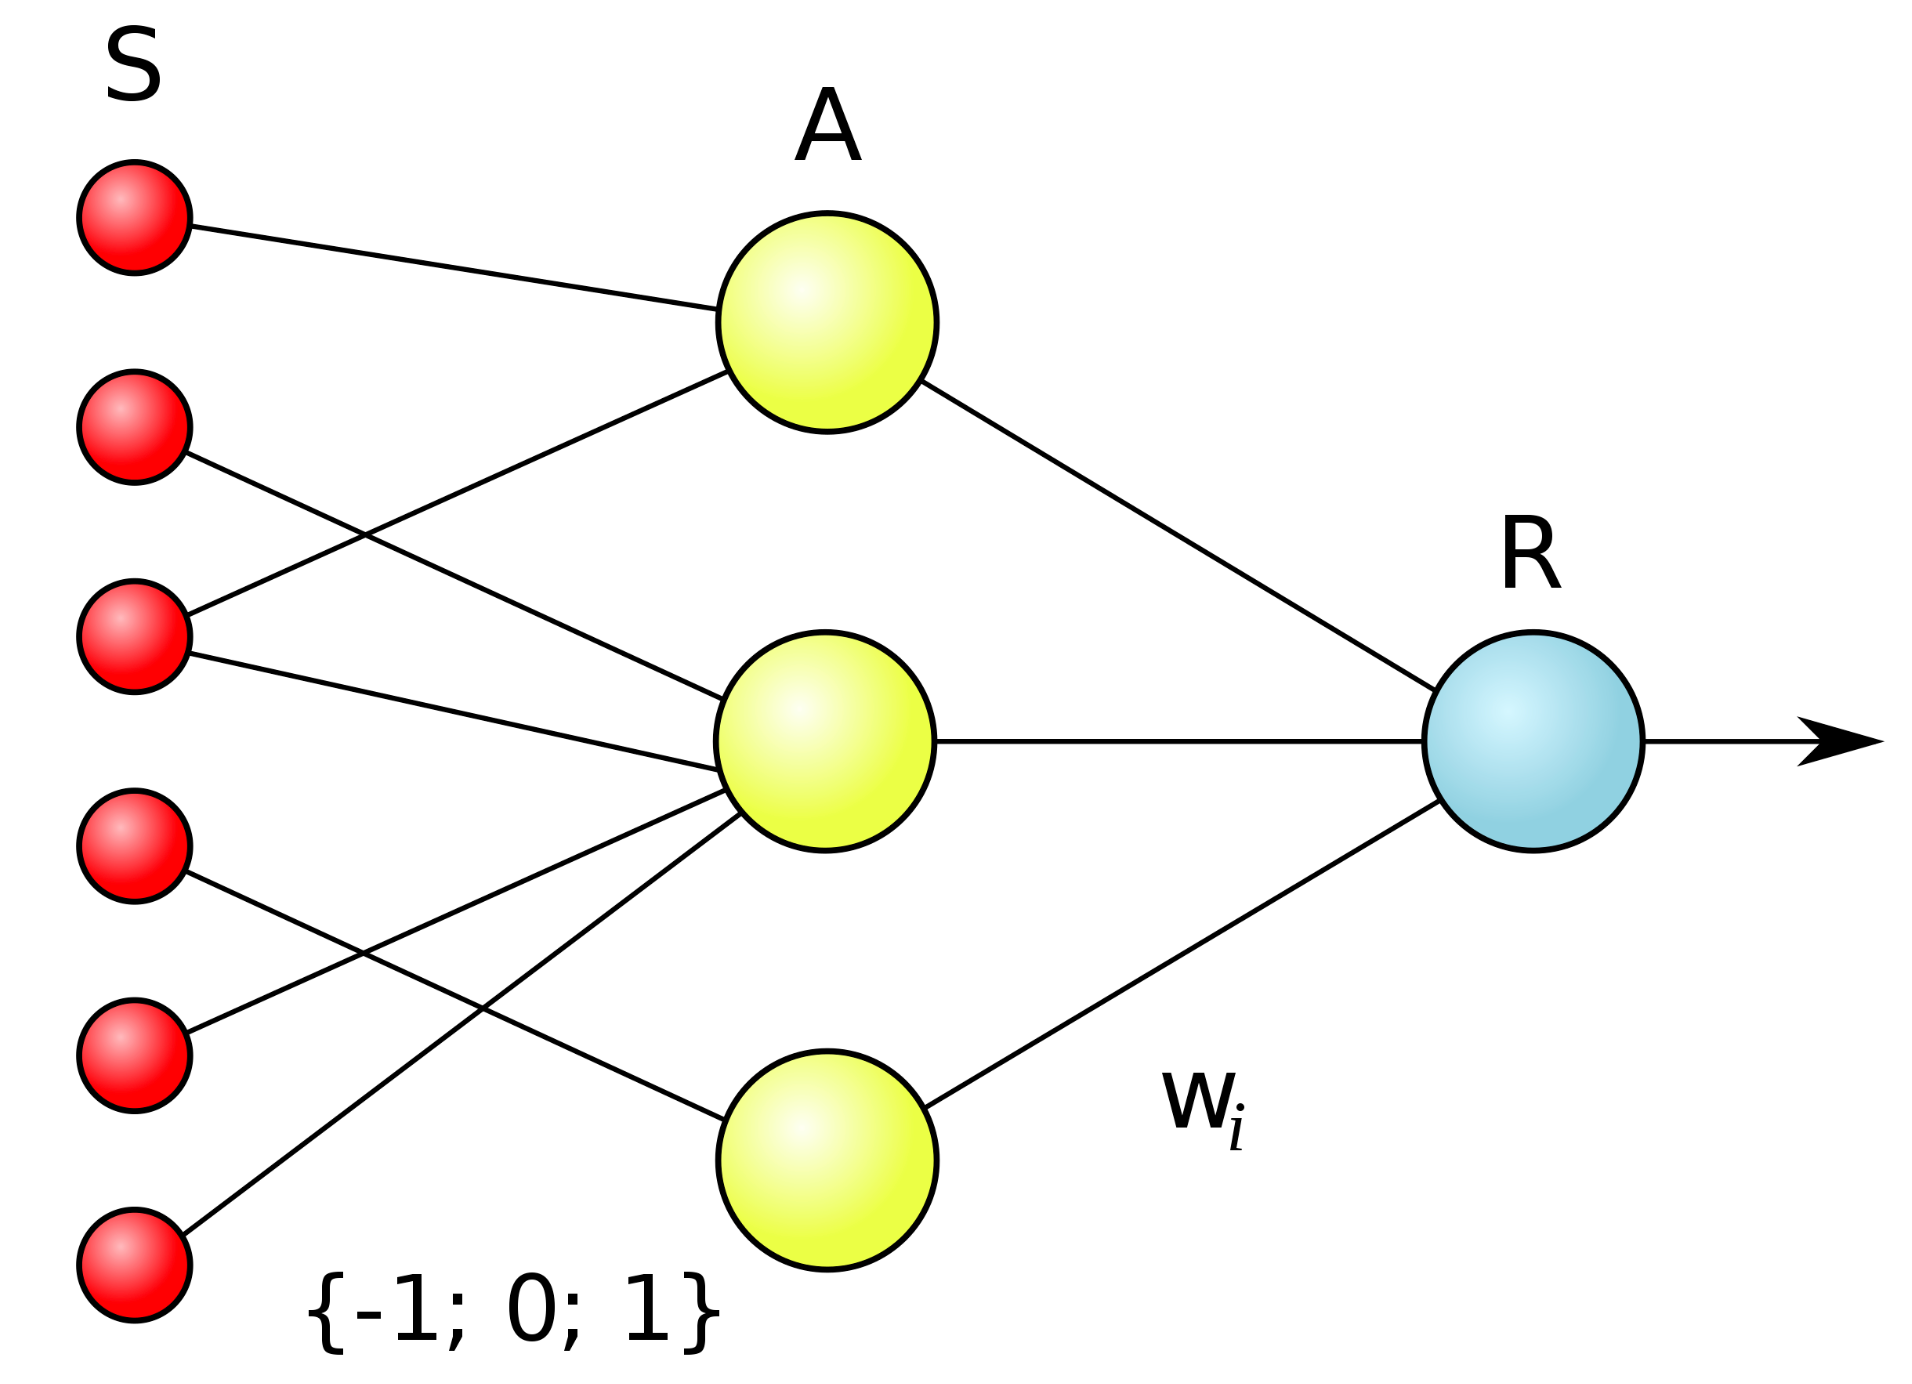
\includegraphics[width=0.6\textwidth]{images/LogicalPerceptron.png}
    \caption{Логічна схема елементарного перспетрону.}
\end{figure}
А-елементи називаються асоціативними, оскільки кожен такий елемент, як правило, відповідає цілому набору (асоціацій) S-елементів. А-елемент активується, як тільки кількість сигналів від S-елементів на його вході перевищила певне значення $\theta$.

Сигнали від збуджених А-елементів, у свою чергу, передаються на суматор R, кожен сигнал із i-того елемента передається із коефіцієнтом $ w_{i}$. Цей коефіцієнт називається вагою зв'язків A-R.

R-елемент обчислює суму значень вхідних сигналів, помножених на вагу (лінійна форма). R-елемент, а разом з ним і елементарний перцептрон, видає $1$, якщо сума перевищує поріг.

Навчання елементарного перцептрона полягає у зміні коефіцієнтів ваг $w_i$  звя’зків A-R. Ваги з'єднань S-A (які можуть приймати значення $[-1; 0; +1]$) та значення порогів A-елементів вибираються випадковим чином на самому початку, а потім не змінюють.

Багатошарова нейронна мережа - це нейронна мережа, що складається з вхідного шару, виходу та розташованих прихованих шарів нейронів (Рис. 3.2).
Такі мережі мають значно більші можливості, ніж персептрон, однак методи навчання нейронів прихованого шару були розроблені порівняно недавно.

Розглянемо це перетворення на прикладі лінійної регресії. Візьмемо $ X $ за вхідний вектор, зміщення $b$, вектор вагів $W$ і оцінку виходу $\hat{y}$.
\[\hat{y}=b + W^{T}X\]


Мінімізуючи функцію втрати, наприклад, MSE ми шукаємо оптимальне рішення.По мірі навчання будее зменшуватись різниця між нашою оцінкою $\hat{y}$ та реальним значенням $y$. Іншими словами, неоптимальні параметри призводять до більших втрат, ніж оптимальні параметри. У нейронній мережі прямого поширення ми використовуємо деяку функцію активації $a$:
\[\hat{y}=a(b + W^{T}X)\]
\begin{figure}
    \centering
    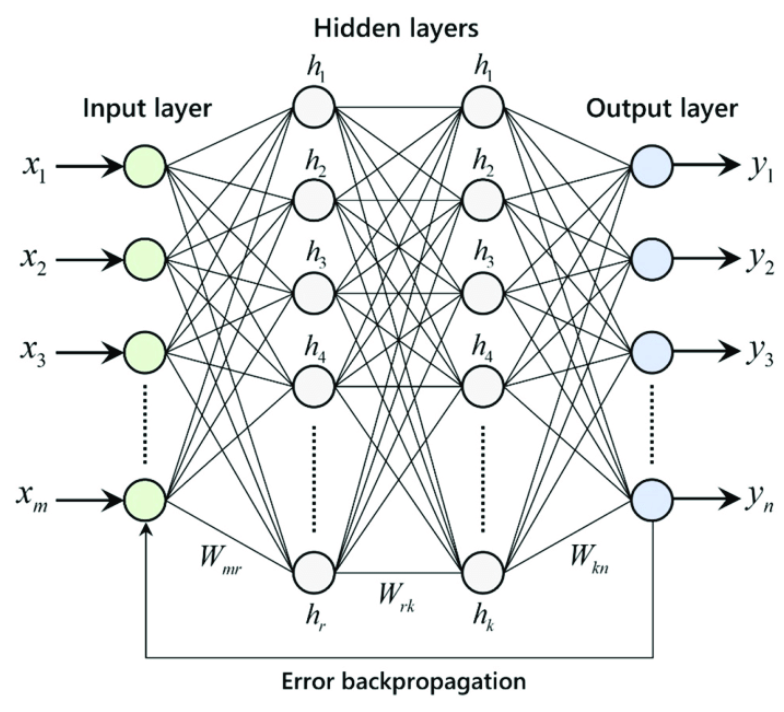
\includegraphics[width=0.4\textwidth]{images/MNN.png}
    \caption{Багатошарова нейронна мережа}
\end{figure}
Нелінійність надає моделі більшу гнучкість, шукаючи глобальний оптимум. Для еффективної роботи моделі нам потрібні ітераційні методи оптимізації.

Одним із найефективніших методів на сьогоднішній день є градієнтний спуск.
Глибокі нейронні мережі (DNN) зазвичай виконують міні-пакетний стохастичний спуск. Цей метод розбиває повну партію тренувань на частини (спліти), які збільшують частоту оновлення порівняно із навчанням на усіх даних (усіма навчальними зразками).

Алгоритим складається із прямого(forward propagation) і зворотнього проходу(backward propagation). На зворотньому проході ми оновлюємо наші параметри (ваги і зміщення) пропорційно обраному коефіцієнту $\alpha$.

\subsection{Автоенкодер}

Генеративні моделі знайшли своє використання у задачах
комп’ютерного зору та обробки природної мови.

Але останні дослідження показали що їх використання не обмежується тільки вищезгаданими сферами. У контексті побудови рекомендацій автоенкодери знайшли рішення групі важливих завдань.

До побудови рекомендацій можливо підійти як до завдання великих даних,внаслідок надзвичайно великого обє’му даних які генерються користувачами (так званий інформаційний слід). Але, із іншої сторони, ці дані в більшості випадків є ненасичені (користувачі взаємодіють лише із мізерною кількістю об’єктів). Що ускладнює завдання вивчення і передбачування побажань усіх користувачів. Для того щоб еффективно інтерпритувати розріджені сигнали було представлено ймовірносну модель засновану на Баєсовій статистиці яка здатна навчатись і поширюватись на скудно насичених даних.

\begin{figure}
    \centering
    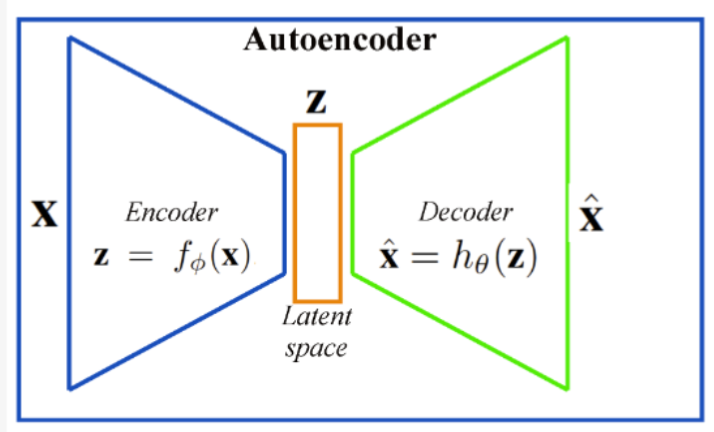
\includegraphics[width=0.7\textwidth]{images/Autoencoder.png}
    \caption{Архітектура нейронної мережі автоенкодера.}
\end{figure}
Автоенкодер у своєму класичному виді - це група із двох моделей глибоких нейронних мереж які використовуються для задачі кодування і декодування вхідних даних (Рис. 3.2).
Це кодування можна сприймати як один із способів зниження розмірності і комплексності вхідного датасету. Що, спрощує структуру моделей і полегшує швидкість навчання череез меншу кількість гіперпараметрів. Для низькорівневого умовного прикладу автоенкодера можна використати  алгоритм аналізу головних компонент (PCA). Ідея якого, це побудова нових признаків більш низької розмірності на основі лінійних комбінацій векторів базавого набору. Під час пошуку найкращої лінійної підмножини алгоритм мінімізує втрати інформації (Рис 3.3).


Але алгоритми такого класу суттєво обмежуються вимогами до не лінійності навчального набору, якщо дані лінійно не залежні алгоритм не знайде їх відображення - тому що його банально не існує.
\begin{figure}
    \centering
    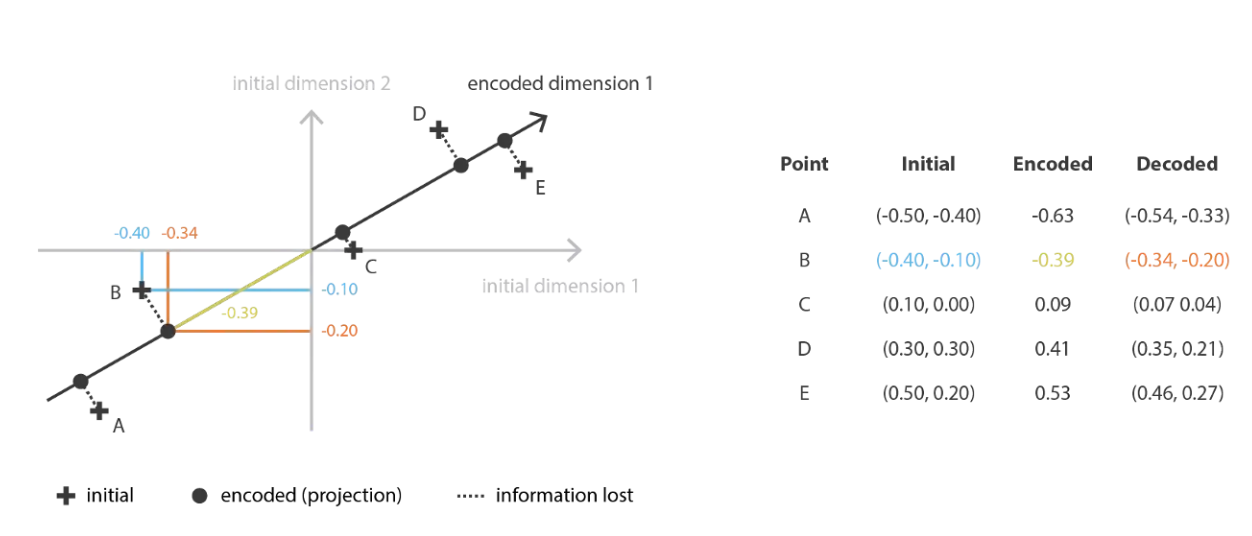
\includegraphics[width=1\textwidth]{images/PCA.png}
    \caption{PCA шукає найкраще відображення вхідних даних у лінійний підпростір меншого розміру}
\end{figure}
Внаслідок чого, були створені алгоритми де у якості енкодера і декодера використовуютсья нейронні мережі для пошуку найкращої функції ітераційним процесом оптимізації. Такий підхід також дозволяє не тільки ефективно кодувати простір, а і зберегти під час стискуваня важливу структурну інформацію.

Завдання навчання автоенкодера у класичному виді можна поставити наступним чином. Нехай $\mathbb{X} \in \mathbb{R}^{m}$ і $\mathbb{Z}\in \mathbb{R}^{n}$ є множини декодованих і закодованих об’єктів відповідно. А $E_{\phi}: \mathcal{X} \to \mathcal{Z} $ і $\mathcal{D}_{\theta}: \mathcal{Z} \to \mathcal{X}   $ деякі сімейства функцій енкодера і декодера пареметризовані $\phi$ і $\theta$ відповідно. Кожен $x \in \mathcal{X}$ вважається закодованим об’єктом при ${z}=\mathbb{E}_{\phi}(x)$ і декодованим (відновленим) при $z \in \mathcal{Z}, x^{\prime} = \mathbb{D}_{\theta}({z})$.

Також введемо функцію $d:\mathcal{X} \times \mathcal{X} \to [0, \infty]$ таку, що $d(x,x^{\prime})$ вимірює наскільки $x^{\prime}$ відрізняється від $x$.

Функція втрат автоенкодера наступна:

\[L(\theta ,\phi ):=\mathbb {\mathbb {E} }_{x\sim \mu {ref}}[d(x,D_{\theta }(E_{\phi }(x)))]\]

Тоді оптимізацію градієнтним спуском ${\displaystyle \arg \min _{\theta ,\phi }L(\theta ,\phi )}$ будемо називати як навчання автоенкодера. А у випадку коли функція $d$ є евклідовою нормою (L2) функція втрат приймає наступний вигляд:

\[ \min _{\theta ,\phi }L(\theta ,\phi ),{\text{where }}L(\theta ,\phi )={\frac {1}{N}}\sum _{i=1}^{N}\|x_{i}-D_{\theta }(E_{\phi }(x_{i}))\|_{2}^{2}\]

У практичних реалізаціях використовують стандартний багатошаровий персептрон (MLP). Принцип його навчання є загально відомий і детального розгляду не потребує. У експериментальній частині буде наведено довідкову інформацію про практичну реалізацію.
\begin{figure}
    \centering
    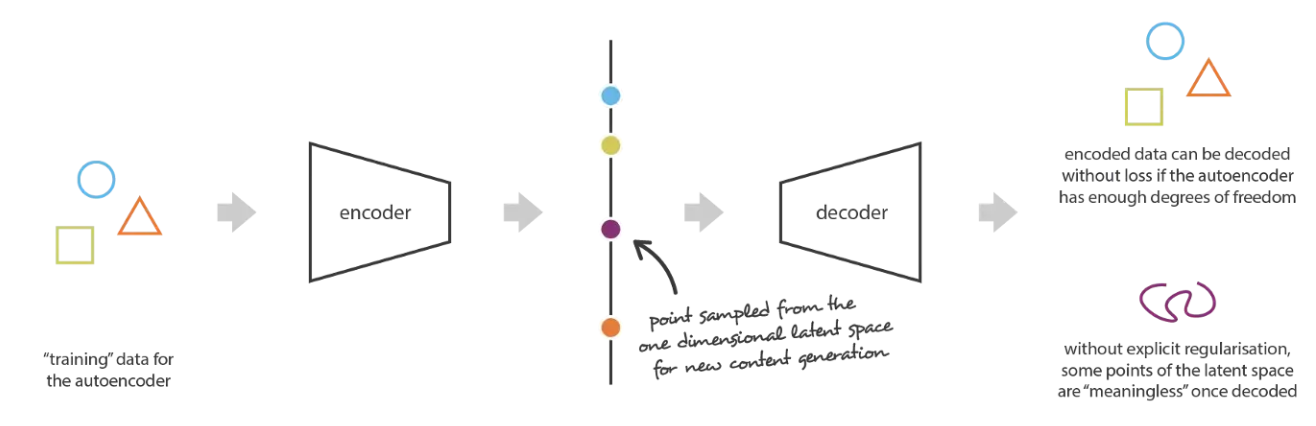
\includegraphics[width=1\textwidth]{images/AE_reg_problem.png}
    \caption{Не регуляризований простір кодування звичайного автоекодера має проблему при використанні в завданнях генерації нових об’єктів.}
\end{figure}
Розглянувши класичну структуру автоенкодера ми перейдемо до найбільш успішної його варіації - Варіаційного автоекодера, що показала прекрасні результати і є лідером у багатьох топ-чартах моделей побудови рекомендацій. Такий розвиток є наслідком Баєсового варіаційного підходу, що дає можливість навчатись не тільки на відомих реальних об’єктах а і на згенерованих самою моделею після вивчення і моделювання потрібного розподілу даних.

Також, однією із причині викоистання такого підходу є не регуляризованість простору прихованих змінних автоенкодера. На Рисунку 3.5 показана інтерпретація цієї проблеми.

Головна особливість варіаційного автоекодера є те, що він вчиться кодувати не вхідний сигнал мережі, а розподіл векторів прихованого простіру(коду).

Отже можна визначити наступні переваги автоенкодерів у завданнях рекомендацій:
\begin{itemize}
    \item Навідмінно від класичних моделей які можуть використовувати тільки один із джерел даних (оцінки взаємодії або текст) автоенкодери використовують широкий спектр гетерогенних даних таких як: оцінки, аудіо, зображення або відео.
    \item Автоенкодер через свою нелінійність краще вивчає вподобання користувачів, що призводить до більш високих оцінок метрик якості.
    \item Автоенкодер адаптивний до багатьох сценаріїв і більш ефективний у випадку боротьби із вхідним шумом у даних.
\end{itemize}
\subsection{Графові нейронні мережі}
Графові нейронні мережі - класс нейронних мереж які оперують даними у вигляді графів (Рис. 3.6). У більш широкому розумінні такий клас мереж можна віднести до геометричного глибинного навчання, в якому існуючі архітектури інтерпретують як графові нейронні мережі. Як приклад - у контексті комп’ютерного зору, зображення можна сприймати як граф пікселів, а у випадку обробки мови, графом представляють слова у тексті. 
До недавного часу більшість моделей векторизації графів були повільні і використовували  алгоритми на основі матричної факторизації або спектральної декомпозиції графів. Однак, додатково вони мали обмеження у використанні, при побудові графу, додаткової інформації, яка могла зберігатись у ребрах або вершинах. Поява графових нейронних мереж стала логічним подальшим розвитком досліджень у сфері побудови графових моделей і дозволило уніфікувати в один підхід минулі розробки.

\begin{figure}
    \centering
    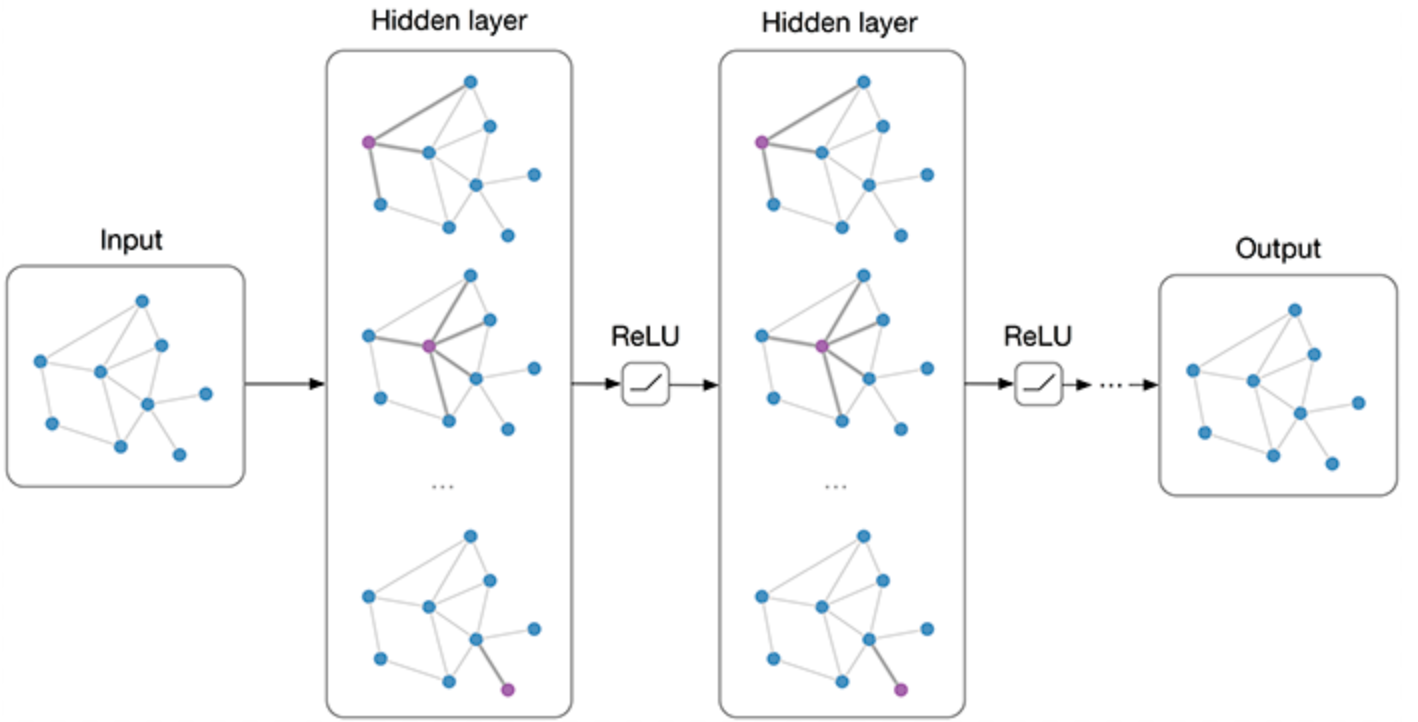
\includegraphics[width=0.8\textwidth]{images/GNN.png}
    \caption{GNN - тип нейронних мереж які напряму працюють із структурою графу.}
\end{figure}


В основі GNN лежить використання механізму передачі повідомлень (Message passing). Граф оброблюється набором модулів, які повязані між собою у відповідності до вузлів графу. Також, кожен із модулів пов’язаний із самими вузлами графа. Під час процесу навчання, модулі обновлюють свої стани і обмінюються інформаціюєю. 
Цей процес відбувається до моменту, поки модулі не перейдуть у стан рівноваги. Вихід GNN обчислюється на базі значень модулів кожного вузла графу.

Нехай, $\mathcal{G} = (\mathcal{V}, \mathcal{E})$ вхідний граф із набором признаків вершин $X \in \mathbb{R}^{d \times |\mathcal{V}|}$. І стоїть завдання побудувати латентне відображення $h_u$  для кожної $u \in\mathcal{V}$. На кожній ітерації GNN, відображення $h_u$ оновлюється агрегацією сигналів
із суміжних вершин  $\mathcal{N}_u$ (Рис. 3.7):
\[ h_u^{k + 1} = f_1^{k}(h_u^{k}, f_2^{k}({h_v^{k}, \forall v \in \mathcal{N}(u)}))\]
\begin{figure}
    \centering
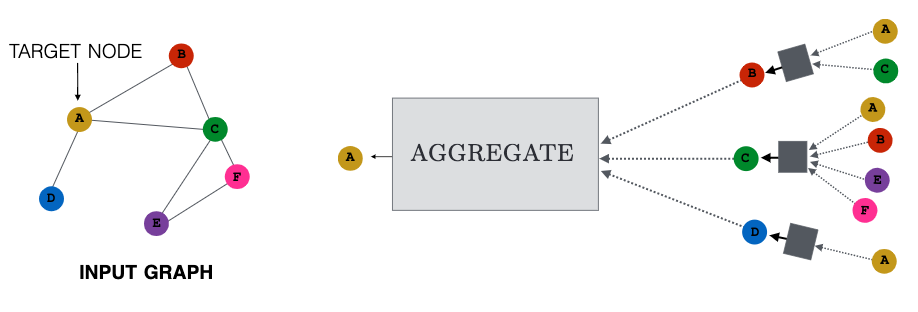
\includegraphics[width=0.8\textwidth]{images/Message_passing.png}
\caption{Ілюстрація агрегації сигналів сусідів для однієї вершини графу. Значення агрегації усереднюються.}
\end{figure}
де $f_1$ і $f_2$ відповідають за операцію оновлення і агрегації, які підбирають в залежності від ситуації. Повідомленням у графових нейронних мережах принято називати:
\[ m_{\mathcal{N}(u)} = f_2^{k}({h_v^{k}, \forall v \in \mathcal{N}(u)})\]

На кожній ітерації $k$, GNN $f_2$ - функція агрегації приймає на вхід набір прихованих значень сусідів, а функція $f_1$ оновлює ембединг об’єкту використовуючи повідомлення $m_{\mathcal{N}(u)}$ і значення із попередньої ітерації $h_k^{u}$.  Після  $K$ ітерацій message passing, ми отримуємо фінальні значення для кожної вершини на вихідному шарі:
\[z_u = h_u^{K}, \forall u \in \mathcal{V}\]
Під ітерацією $k$ можна розуміти глибину передачі повідомлень, чим він більший, тим більша відстань від $u$ до вершин які агрегуються. Такий підхід має ціль зібрати інформацію про структуру сусідніх елементів, а також про значення признаків їх вершин.

У разі використання моделі персептрону  Рів. 2.6 приймає наступний вигляд:
\[ h_u^{k} = \sigma \left(W_{self}^{k} h_u^{k-1} + W_{neigh}^{k} \sum_{v \in \mathcal{N}(u)} h_v^{k-1} + b^{k}\right)\]
де $W_{self}^{k}$ і $W_{neigh}^{k}$ матриці вагів мережі, а $\sigma$ не лінійна функція активації.

Графові нейронні мережі у задачах побудови рекомендацій знайшли своє використання у таких завданнях:

\begin{itemize}
    \item \textbf{Рекомендація послідовностей (Sequential Recommendation)}. Аналізуючи послідовнісь дій користувачів, такі моделі хочуть на основі деякого ланцюга подій  ${x_1, x_2, ..., x_n}$ довжини $n$ передбачити $x_{n+1}$ об’єкт (Рис 3.8).
    \item \textbf{Рекомедація на основі сесії}. Одна із найскладніших завдань. У моделі стоїть ціль передбачити $x_{n+1}$ об’єкт на основі активної сесії користувача, тобто в режимі реального часу.
    \item \textbf{Соціальні рекомендації}. Великі соціальні мережі використовують моделі для передбачування поведінки і побажань своїх користувачів. В майбутньому ці дані можуть бути використані для продажу або реклами (наприклад Facebook Ads).

\end{itemize}

\begin{figure}
    \centering
    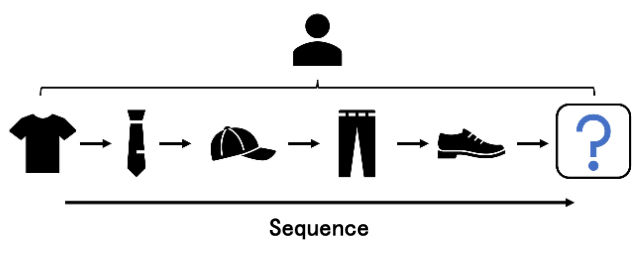
\includegraphics[width=0.8\textwidth]{images/Seq_rec.png}
    \caption{Ілюстрація завдання передбачення послідовності.}
    \end{figure}
\subsection*{Висновок}
У розділі розглянуто принцип роботи нейронної мережі прямого поширення на прикладі персептрону. Проаналізовано аріхтектури нейромереж на основі автоекодера і графової нейронної мережі. Розглянуто ключові деталі їх роботи: алгоритм навчання автоенкодера і механізм передачі повідомлень. Розглянуто принцип роботи і основні переваги використання вищезгаданих архітектур у завданнях побудови рекомендацій.